\part{Développement}
\section{Justification des choix techniques}

	\subsection{Netbeans}

	\href{https://netbeans.org/}{Netbeans} est un IDE. Un IDE est un Environnement de Développement Intégré. Il fournit tous les outils nécessaires pour implémenter notre projet.

	Nous avons choisi Netbeans pour sa bonne intégration avec Glassfish : le serveur est directement contrôlable et débuggable depuis Netbeans.

	\subsection{Git}

		\href{http://git-scm.com/}{Git} est un logiciel de gestion de versions. Il nous permet de gérer différentes versions concurrentes de notre code.

		Git nous a permis de travailler ensemble sur ce projet.

	\subsection{Bootstrap}

		\href{http://getbootstrap.com/}{Bootstrap} est un framework CSS. Il s'agit d'un ensemble de règles définissant l'apparence de notre page web.

		Utiliser Bootstrap nous permet de nous concentrer sur la structure de nos pages, plutôt que de créer nous-même nos styles alors que notre temps est déjà limité.

\section{Procédures de tests}


\clearpage
\section{Conception UML}
	\subsection{Diagramme de cas d'utilisation}
	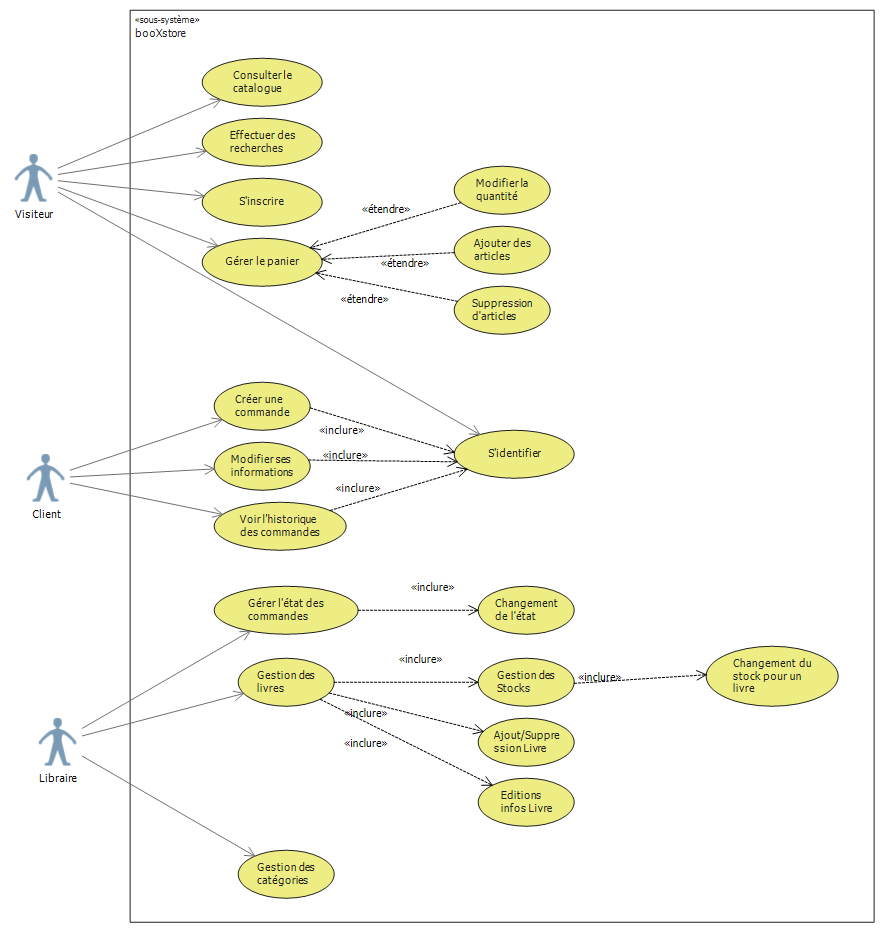
\includegraphics[scale=0.4]{Res/useCase.png}
	Le diagramme des cas d'utilisation a été crée pour nous fournir une représentation visuelle des relations entre les différentes fonctionnalités de l'application ; ainsi que de nous fournir un récapitulatif de ces dernières. \\

	Nous voyons ici que l'utilisateur lambda a accès à la consultation du catalogue, aux fonctions de recherche, à l'inscription, à la gestion de son panier(comprenant la modification de la quantité des articles contenus, l'ajout / la suppression d'articles)

	L'utilisateur peut également décider de se connecter / s'inscrire pour devenir client, ce qui lui donnera accès aux fonctions de création de commande, de modification des informations personnelles ainsi qu'a celles d’affichage de l'historique des commandes

	\clearpage
	\subsection{Diagramme d'activité}
	\includegraphics[scale=0.5]{Res/activityCOmmande.png} \\
	Le diagramme d'activité récapitule l’intégralité des actions à effectuer par l'utilisateur afin de créer une nouvelle commande. \\

	Une fois le panier rempli, l'utilisateur va demander à le valider. Cette validation va lancer la création de la commande. Si l'utilisateur n'est pas connecté, l'application va demander à l'utilisateur de se connecter.

	Si l'utilisateur était connecté, alors on passe à la phase de remplissage des données bancaires. Une fois saisies, les données sont vérifiées. Le client devra ressaisir des coordonnées bancaire jusqu’à ce qu'elles soient valides.

	Une fois cette vérification effectuée, la commande est enregistrée.

	\clearpage
	\subsection{Diagrammes de séquences}
	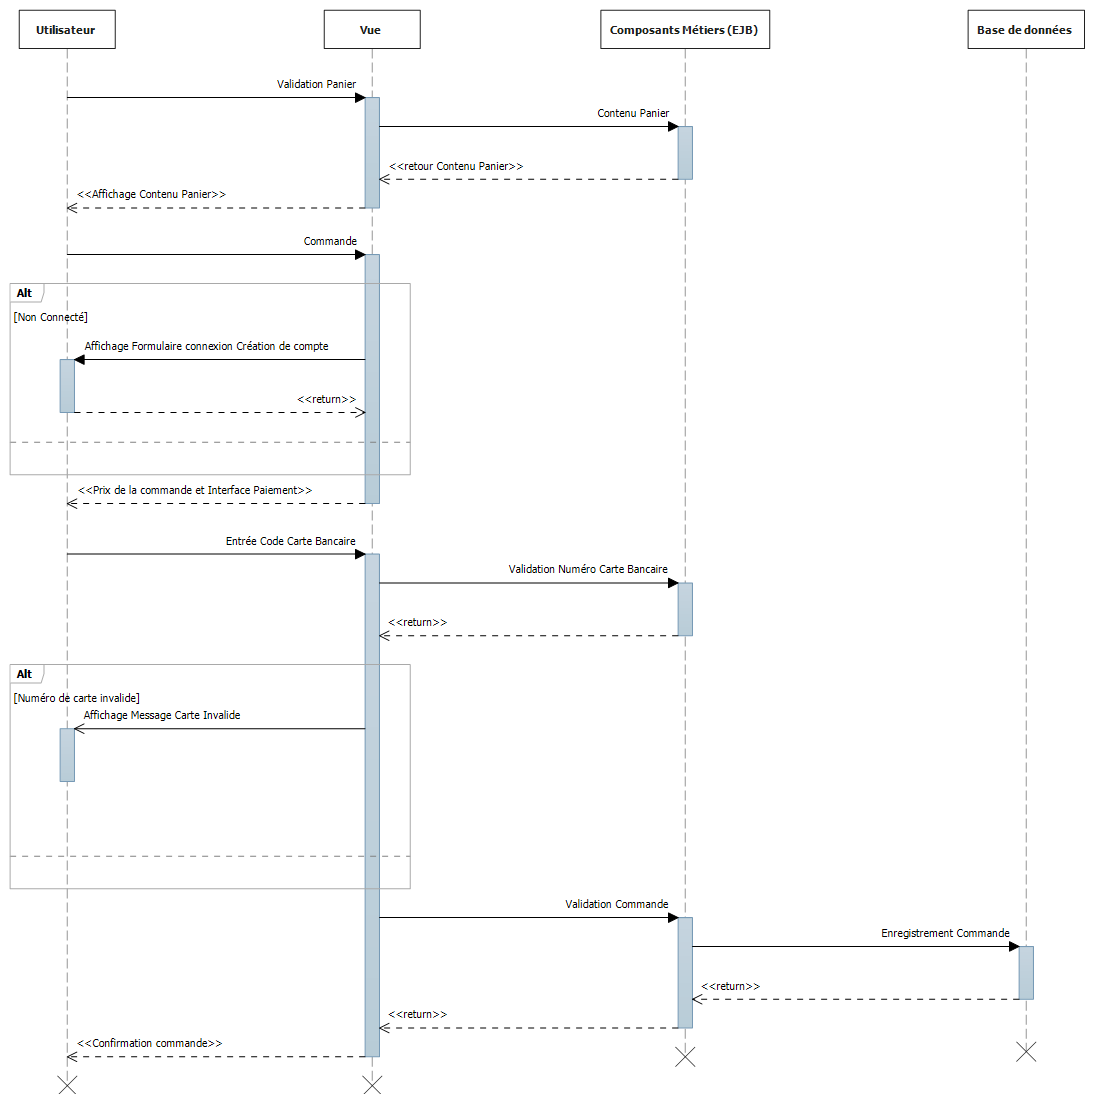
\includegraphics[scale=0.39]{Res/sequenceDiagramOrder.png}
	Ce diagramme de séquence décrit les interactions entre les différentes couches de l’application nécessaires pour la création d'une commande. \\

	Une fois la validation du panier effectuée par le client, le signal de validation est envoyé à la vue. Vue qui demande le contenu du panier au composant métier dédié.

	Le client valide alors sa commande. S'il n'est pas connecté, la Vue lui affiche alors le formulaire de connexion / inscription. Une fois la connexion faite la Vue demande à l'utilisateur de rentrer ses informations bancaires. Si le numéro entré est invalide, on affiche un message d'erreur  à l'utilisateur et on redemande la saisie.

	Si le numéro est validé, on envoie un message de validation de la commande au composant métier qui va enregistrer la commande en base de données.

	Une fois la commande enregistrée, la base renverra une confirmation au composant métier qui renverra lui même une confirmation à la vue qui informera l'utilisateur de la réussite de l'opération.

	\clearpage
	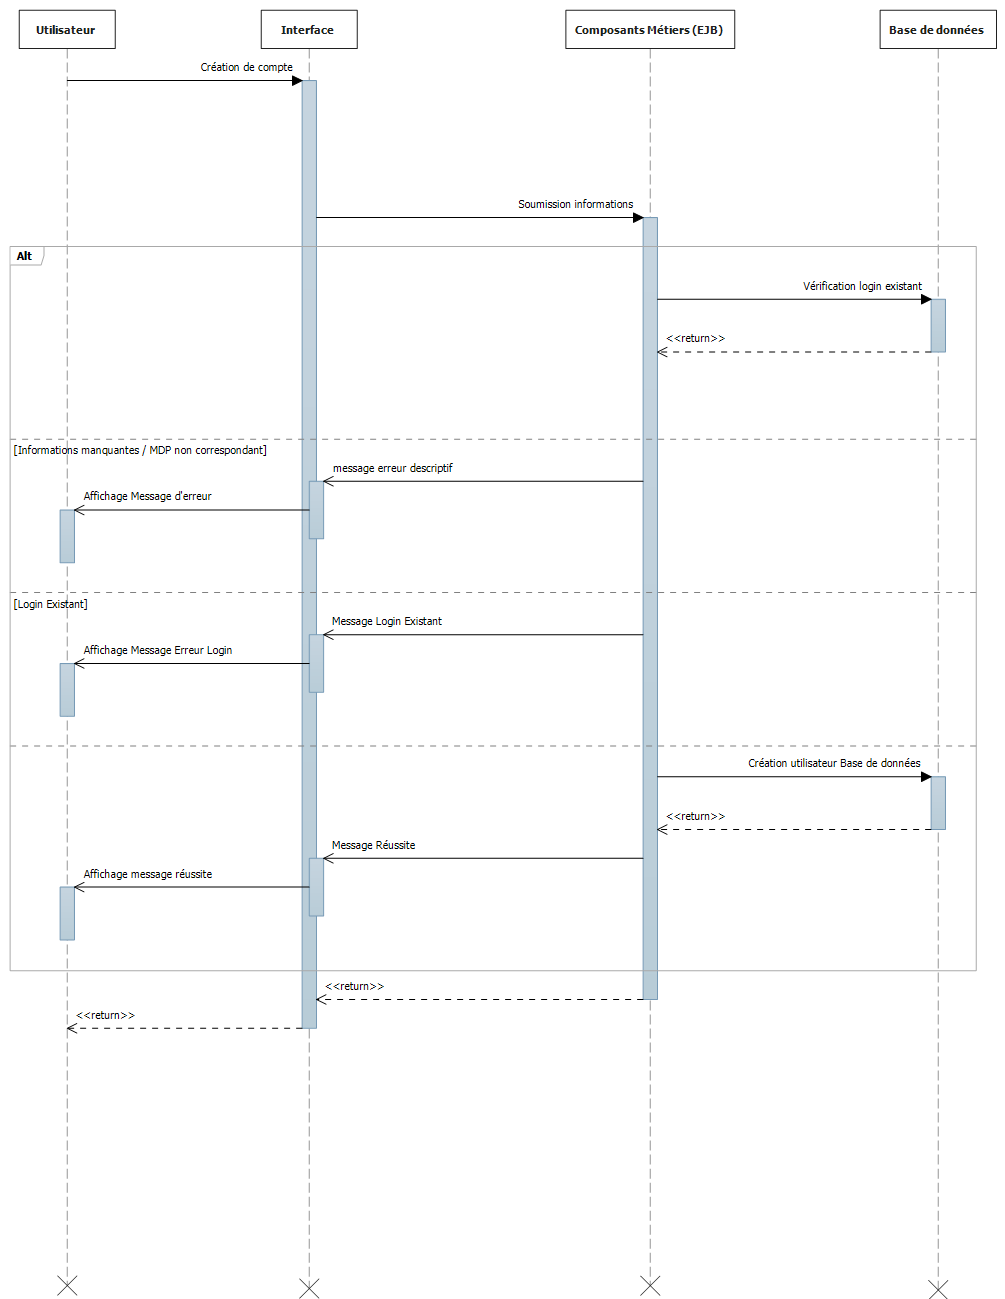
\includegraphics[scale=0.37]{Res/accountCreationSequence.png}
	Ce diagramme de séquence décrit les interactions entre les différentes couches de l'application nécessaires pour la création d'un compte utilisateur. \\

	Une fois que l'utilisateur a inscrit ses données dans le formulaire d'inscription, l'interface soumet les informations au composant métier qui va vérifier en base si le login existe déjà.

	S'il existe, le composant métier renverra un message à la vue qui affichera un message d'erreur à l'utilisateur qui devra choisir un login différent.

	Si une autre erreur est détectée, l'interface l'affichera de la même manière.

	Si les informations sont correctes, le composant métier créera l'utilisateur en base et en informera la vue qui à son tour en informera l'utilisateur.

	\clearpage
	\subsection{Diagramme de classes}
	Au vu de la taille du diagramme, il se peut que celui-ci ne soit pas lisible sur une feuille A4, voici un lien pour le télécharger à part : \href{http://goo.gl/D9HGij}{http://goo.gl/D9HGij}

\section{Points forts et points faibles de notre implémentation}

	\subsection{Points forts}
	\begin{itemize}

		\item L'ergonomie. Le site a été conçu avec Bootstrap. Il s'agit d'un framework CSS : il va gérer l'apparence de nos pages à notre place. Ceci nous à permis de nous concentrer sur la structure et l'ergonomie. Par exemple :

		\begin{itemize}
			\item La barre de navigation. Celle-ci permet - comme son nom l'indique - de naviguer dans notre site. Elle fournit des informations utiles à l'utilisateur, comme le contenu de son panier. On peut également effectuer des recherches directement à partir de celle-ci.

			\item Le site est \emph{responsive}. Cela signifie que l'affichage s'adapte à la taille de l'écran de l'utilisateur. Ainsi, que celui-ci utilise un smartphone, une tablette, un laptop, ou même un écran plus large, le contenu sera toujours disposé de façon optimale pour lui.
		\end{itemize}

		\item La partie client s'exécute rapidement. Couplé à une bonne ergonomie, cela offre à nos utilisateurs une expérience très fluide.

	\end{itemize}


	\subsection{Points faibles}
	\begin{itemize}
		\item Le catalogue n'affiche pas de résultats par défaut. Autrement dit, il faut effectuer une recherche pour afficher des livres.

		\item La page de gestion n'est pas paginée, comme peut l'être le catalogue par exemple. Dans le cas d'un nombre important de livres, l'affichage peut être ralentit.
	\end{itemize}
